\documentclass[a4paper, 10pt, twoside]{article}

\usepackage[top=1in, bottom=1in, left=1in, right=1in]{geometry}
\usepackage[utf8]{inputenc}
\usepackage[spanish, es-ucroman, es-noquoting]{babel}
\usepackage{setspace}
\usepackage{fancyhdr}
\usepackage{lastpage}
\usepackage{amsmath}
\usepackage{amsfonts}
\usepackage{amsthm}
\usepackage{verbatim}
\usepackage{graphicx}
\usepackage{float}
\usepackage[noend]{algpseudocode}
\usepackage{enumitem} % Provee macro \setlist
\usepackage[toc, page]{appendix}


%%%%%%%%%% Configuración de Fancyhdr - Inicio %%%%%%%%%%
\pagestyle{fancy}
\thispagestyle{fancy}
\lhead{Trabajo Práctico 3 · Algoritmos y Estructuras de Datos III}
\rhead{Lovisolo · Petaccio · Rossi}
\renewcommand{\footrulewidth}{0.4pt}
\cfoot{\thepage /\pageref{LastPage}}

\fancypagestyle{caratula} {
   \fancyhf{}
   \cfoot{\thepage /\pageref{LastPage}}
   \renewcommand{\headrulewidth}{0pt}
   \renewcommand{\footrulewidth}{0pt}
}
%%%%%%%%%% Configuración de Fancyhdr - Fin %%%%%%%%%%


%%%%%%%%%% Configuración de Algorithmic - Inicio %%%%%%%%%%
% Entorno propio para customizar la presentación del pseudocódigo
\newenvironment{pseudo}[1][]{%
    \vspace{1em}%
    \begin{algorithmic}%
}
{%
    \end{algorithmic}%
    \vspace{1em}%
}


% switch
\algnewcommand\algorithmicswitch{\textbf{switch}}
\algnewcommand\algorithmiccase{\textbf{case}}
\algnewcommand\algorithmicassert{\texttt{assert}}
\algdef{SE}[SWITCH]{Switch}{EndSwitch}[1]{\algorithmicswitch\ #1\ \algorithmicdo}{\algorithmicend\ \algorithmicswitch}%
\algdef{SE}[CASE]{Case}{EndCase}[1]{\algorithmiccase\ #1}{\algorithmicend\ \algorithmiccase}%
\algtext*{EndSwitch}%
\algtext*{EndCase}%




% Valores de verdad
\newcommand{\True}{\textbf{true}}
\newcommand{\False}{\textbf{false}}

% Conectivos lógicos
\newcommand{\PAnd}{\textbf{and} }
\newcommand{\POr}{\textbf{or} }

% Conectivo 'in' para usar así: \ForAll{$foo$ \In $bar$}
\newcommand{\In}{\textbf{in} }

% Conectivo 'to' para usar así: \For{$i = 1$ \In $n$}
\newcommand{\To}{\textbf{to} }

% Control de flujo
\newcommand{\Break}{\State \textbf{break}}
\newcommand{\PReturn}{\State \textbf{return} }

% Complejidades
\newcommand{\Ode}[1]{\hfill $O(#1)$}
%%%%%%%%%% Configuración de Algorithmic - Fin %%%%%%%%%%


%%%%%%%%%% Miscelánea - Inicio %%%%%%%%%%
% Evita que el documento se estire verticalmente para ocupar el espacio vacío
% en cada página.
\raggedbottom

% Deshabilita sangría en la primer línea de un párrafo.
\setlength{\parindent}{0em}

% Separación entre párrafos.
\setlength{\parskip}{0.5em}

% Separación entre elementos de listas.
\setlist{itemsep=0.5em}

% Asigna la traducción de la palabra 'Appendices'.
\renewcommand{\appendixtocname}{Apéndices}
\renewcommand{\appendixpagename}{Apéndices}
%%%%%%%%%% Miscelánea - Fin %%%%%%%%%%


%%%%%%%%%% Gráficos - Inicio %%%%%%%%%%
% Macro para incluir tres gráficos (dentro de una figura) de manera que
% entren todos en una sola página.
\newcommand{\tresgraficos}[3]{
    \newcommand{\separacion}{-2.2em}
    \vspace{\separacion}
    \include{#1}
    \vspace{\separacion}
    \include{#2}
    \vspace{\separacion}
    \include{#3}
}

% Macro para incluir dos gráficos (dentro de una figura) de manera que
% entren todos en una sola página.
\newcommand{\dosgraficos}[2]{
    \newcommand{\separacion}{-2.2em}
    \vspace{\separacion}
    \include{#1}
    \vspace{\separacion}
    \include{#2}
}
%%%%%%%%%% Gráficos - Fin %%%%%%%%%%


\begin{document}


%%%%%%%%%%%%%%%%%%%%%%%%%%%%%%%%%%%%%%%%%%%%%%%%%%%%%%%%%%%%%%%%%%%%%%%%%%%%%%%
%% Carátula                                                                  %%
%%%%%%%%%%%%%%%%%%%%%%%%%%%%%%%%%%%%%%%%%%%%%%%%%%%%%%%%%%%%%%%%%%%%%%%%%%%%%%%


\thispagestyle{caratula}

\begin{center}


\includegraphics[height=2cm]{DC.png} 
\hfill

\includegraphics[height=2cm]{UBA.jpg} 

\vspace{2cm}

Departamento de Computación,\\
Facultad de Ciencias Exactas y Naturales,\\
Universidad de Buenos Aires

\vspace{4cm}

\begin{Huge}
Trabajo Práctico 3
\end{Huge}

\vspace{0.5cm}

\begin{Large}
Algoritmos y Estructuras de Datos III
\end{Large}

\vspace{1cm}

Segundo Cuatrimestre de 2013

\vspace{4cm}

\begin{tabular}{|c|c|c|}
\hline
Apellido y Nombre & LU & E-mail\\
\hline
Leandro Lovisolo      & 645/11 & leandro@leandro.me\\
Lautaro José Petaccio & 443/11 & lausuper@gmail.com\\
Lucas Rossi           & 705/11 & lucasrossi20@gmail.com\\
\hline
\end{tabular}

\end{center}

\newpage


%%%%%%%%%%%%%%%%%%%%%%%%%%%%%%%%%%%%%%%%%%%%%%%%%%%%%%%%%%%%%%%%%%%%%%%%%%%%%%%
%% Índice                                                                    %%
%%%%%%%%%%%%%%%%%%%%%%%%%%%%%%%%%%%%%%%%%%%%%%%%%%%%%%%%%%%%%%%%%%%%%%%%%%%%%%%


\tableofcontents

\newpage


%%%%%%%%%%%%%%%%%%%%%%%%%%%%%%%%%%%%%%%%%%%%%%%%%%%%%%%%%%%%%%%%%%%%%%%%%%%%%%%
%% Introducción                                                              %%
%%%%%%%%%%%%%%%%%%%%%%%%%%%%%%%%%%%%%%%%%%%%%%%%%%%%%%%%%%%%%%%%%%%%%%%%%%%%%%%


\section{Introducción}

En el presente trabajo estudiamos tres problemas algorítmicos, proponemos soluciones para los mismos respetando sus requerimientos de complejidad temporal y analizamos empíricamente los tiempos de ejecución de sus implementaciones en lenguaje C++.

La motivación de este trabajo es comparar las cotas temporales obtenidas del análisis teórico con las mediciones de tiempos de ejecución y extraer conclusiones de esta experimentación.

Sin más, presentamos los problemas estudiados a continuación.


%%%%%%%%%%%%%%%%%%%%%%%%%%%%%%%%%%%%%%%%%%%%%%%%%%%%%%%%%%%%%%%%%%%%%%%%%%%%%%%
%% Descipcion de situaciones reales                                          %%
%%%%%%%%%%%%%%%%%%%%%%%%%%%%%%%%%%%%%%%%%%%%%%%%%%%%%%%%%%%%%%%%%%%%%%%%%%%%%%%


\newpage

\section{Descripción de situaciones reales}
\begin{itemize}
\item Un área perteneciente a un bosque quiere abrirse a turistas. El bosque tiene una serie de senderos (aristas) que lo recorren y una serie de espacios libres (nodos). Los guardabosques quieren que la gente no se pierda nada de la naturaleza del bosque, quieren que los turistas puedan recorrer la mayor cantidad de caminos posibles. Como la gente es muy vaga, solo recorre los caminos que estén conectados a un claro donde haya un puesto para bebidas y descanso. Es necesario que los puestos estén todos comunicados para poder proveerse entre sí en caso de que a alguno le falte algo o necesite ayuda. 

Mediante el algoritmo de CFM podemos encontrar los espacios libres conectados entre sí para poner los paradores de manera que la gente pueda recorrer la mayor cantidad posible de caminos del bosque sin cansarse tanto.
\end{itemize}

%%%%%%%%%%%%%%%%%%%%%%%%%%%%%%%%%%%%%%%%%%%%%%%%%%%%%%%%%%%%%%%%%%%%%%%%%%%%%%%
%% Algoritmo exacto                                                          %%
%%%%%%%%%%%%%%%%%%%%%%%%%%%%%%%%%%%%%%%%%%%%%%%%%%%%%%%%%%%%%%%%%%%%%%%%%%%%%%%


\newpage

\section{Algoritmo exacto}
\subsection{Algoritmo}
Para la implementación del algoritmo exacto utilizamos la técnica de backtracking que puede verse a continuación.

\begin{pseudo}
\State \textbf{indice\_nodo} es int
\State \textbf{nodo} es tupla $<$ indice\_nodo indice, conjuto$<$indice\_nodo$>$ adyacentes$>$
\State \textbf{cmf} es par$<$frontera : int, indices\_nodos : vector de indice\_nodo$>$
\State
\Procedure{exacto}{\&nodos : vector de nodo} $\rightarrow$ cmf
	\State return exacto\_rec(nodos, vector de indice\_nodo vacío, 0)
\State
\EndProcedure

\Procedure{exacto\_rec}{\&nodos : vector de nodo,
		       \&clique\_inicial : vector de indice\_nodo,
		       pos : unsigned} $\rightarrow$ cmf
	\If{pos == Tamaño(nodos)} return nueva\_cmf(0, vector de indice\_nodo vacío) \EndIf

	\State mejor\_cmf : cmf									\Ode{1}

	\For{i = pos To Tamaño(nodos) -1}
		\If{agregandoSigueSiendoClique(nodos, clique\_inicial, i)} \Ode{N * log N}
			\State agregandoIesimo : cmf $\leftarrow$ nueva\_cmf(0, clique\_inicial)	\Ode{1}
			\State indices\_nodos(agregandoIesimo).Agregar(i)	\Ode{1}
			\State frontera(agregandoIesimo) $\leftarrow$
					cardinalFrontera(nodos, indices\_nodos(agregandoIesimo))	\Ode{N}
			\State subproblema : cmf $\leftarrow$
					exacto\_rec(nodos, indices\_nodos(agregandoIesimo), i + 1)

			\If{frontera(agregandoIesimo) $>$ frontera(subproblema)}
				\State \&candidata : cmf $\leftarrow$ agregandoIesimo			\Ode{N}
			\Else 
				\State \&candidata : cmf $\leftarrow$ subproblema				\Ode{N}
			\EndIf

			\If{frontera(candidata) $>$ frontera(mejor\_cmf)} \Ode{1}
				\State mejor\_cmf $\leftarrow$ candidata	\Ode{N}
			\EndIf
		\EndIf
	\EndFor

	\State return mejor\_cmf
\EndProcedure
\end{pseudo}

\subsection{Complejidad}

\subsection{Pérformance}
%%%%%%%%%%%%%%%%%%%%%%%%%%%%%%%%%%%%%%%%%%%%%%%%%%%%%%%%%%%%%%%%%%%%%%%%%%%%%%%
%% Heurística contructiva golosa                                             %%
%%%%%%%%%%%%%%%%%%%%%%%%%%%%%%%%%%%%%%%%%%%%%%%%%%%%%%%%%%%%%%%%%%%%%%%%%%%%%%%


\newpage

\section{Heurística contructiva golosa}
\subsection{Algoritmo}
La implementación realizada para resolver el problema con una heurística golosa realiza los siguientes procedimientos:
\begin{enumerate}
\item Elijo el nodo de grado máximo que sera la clique de tamaño 1 donde empezara el algoritmo. Marco como actual el nodo inicial.
\item Para el nodo actual, recorro sus adyacentes y calculo cuanto aportaría a la frontera agregar ese adyacente si es posible agregarlo al clique.
\item Agrego al clique el máximo de todos los adyacentes vistos y lo elijo como el actual.
\item Vuelvo al punto 2 hasta que no haya adyacente que mejore la frontera.
\end{enumerate}

A continuación presentamos el pseudocódigo:

\begin{pseudo}
\State \textbf{indice\_nodo} es int
\State \textbf{nodo} es tupla $<$ indice\_nodo indice, conjuto$<$indice\_nodo$>$ adyacentes$>$
\State \textbf{cmf} es par$<$frontera : int, indices\_nodos : vector de indice\_nodo$>$
\State
\Procedure{golosa}{\&nodos : vector de nodo} $\rightarrow$ cmf
	\State clique : cmf														\Ode{1}
	\State actual : indice\_nodo $\leftarrow$ nodoDeMayorGrado(nodos)		\Ode{N}

	\While{true}
	 	\State indices\_nodos(clique).Agregar(actual);						\Ode{1}
	 	\State candidato : indice\_nodo										\Ode{1}
		\State aporteCandidato : int $\leftarrow$ 0							\Ode{1}

	 	\For{it : iterator de nodos[actual].adyacentes ; Begin(it) To End(it)}

	 		\State adyacente : indice\_nodo = *it							\Ode{1}
	 		
	 		\If{agregandoSigueSiendoClique(
	 				nodos, indices\_nodos(clique), adyacente) \&\& \State
	 		   !estaEnLaClique(indices\_nodos(clique), adyacente)}			\Ode{N*log N}

	 			\State aporte : int $\leftarrow$ Tamaño(nodos[adyacente].adyacentes) -
	 					     2 * Tamaño(indices\_nodos(clique))				\Ode{1}

	 			\If{aporte $>$ aporteCandidato}								\Ode{1}
	 				\State aporte : aporteCandidato							\Ode{1}
	 				\State candidato $\leftarrow$ adyacente					\Ode{1}
	 			\EndIf
	 		\EndIf
	 	\EndFor
	 	\If{aporteCandidato $>$ 0} actual $\leftarrow$ candidato			\Ode{1}
	 	\Else
	 		\State break
	 	\EndIf
	\EndWhile

	\State frontera(clique) $\leftarrow$ cardinalFrontera(nodos, indices\_nodos(clique)) \Ode{N}
	\State return clique
\EndProcedure
\end{pseudo}

\subsection{Complejidad}
Sea N cantidad de nodos en el grafo.

En la función estaEnLaClique se tiene un ciclo de a lo sumo N veces (máximo clique), realizando operaciones O(1), por lo que la función tiene una complejidad de O(N).

En el algoritmo goloso, se cicla hasta que cambio sea igual a true. Como el algoritmo solo puede agregar nodos nuevos al clique, se ciclaran a lo sumo N veces.
Dentro del ciclo del while se tiene un for que recorre todos los adyacentes del nodo que a lo sumo puede tener a todos los nodos del grafo como adyacentes, por lo que se cicla N veces.
La complejidad ambos ciclos es N * N * O(N*log N) $\subset$ O($N^3$ * log N).
Para finalizar, tiene un for que cicla a lo sumo N veces realizando operaciones O(1).
La complejidad final del algoritmo es O(N) + O($N^3$ * log N) = O($N^3$ * log N).

\subsection{Análisis de eficacia}
Es posible determinar que el algoritmo goloso se desempeñará de forma ineficaz ante grafos que no incluyan al nodo de mayor grado en el clique de mayor frontera, ya que este siempre formará parte de la solución provista por el algoritmo. Esta solución empeora aun más, como podemos ver en el siguiente gráfico, si el nodo de grado máximo tiene adyacentes de grado 1, haciendo que el algoritmo no pueda explorar el grafo, debido a que al tomarlos como parte del clique solución, no mejorarán la frontera y no se tendran en cuenta.

\begin{figure}[H]
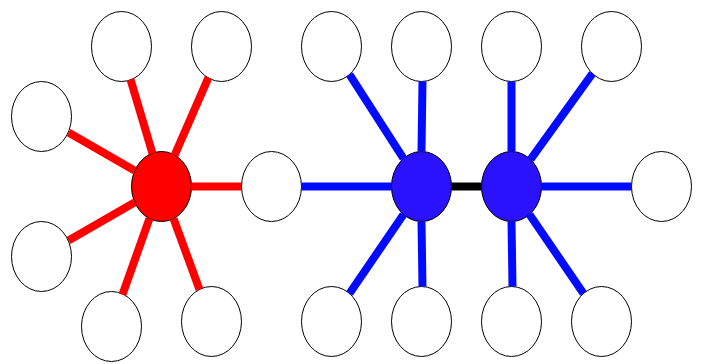
\includegraphics[width=80mm]{ejemploErrorGoloso.png}
\caption{Las aristas de color rojo forman parte de la frontera encontrada por el algoritmo, mientras que las aristas de color azul forman la frontera máxima}
\label{overflow}
\end{figure}

Analizando este grafo, puede encontrarse una familia, la cuál es posible manipular para conseguir una respuesta tan mala como se desee. Esta familia está compuesta por un nodo de grado máximo no incluido en la solución y una clique donde cada nodo tiene grado máximo posible (grado máximo - 1).

Incrementando la cantidad de adyacentes del nodo de mayor grado (nodo de color rojo), podemos hacer que el verdadero clique (parte azul) crezca, pudiendo incrementar la diferencia entre la frontera encontrada por el algoritmo y la frontera máxima del grafo provista por una clique.

Tomando \textbf{d} = nodo de grado máximo y \textbf{c} = tamaño de clique elegido para sección azul, obtenemos que es posible calcular la frontera máxima según el tamaño del clique elejido y del grado máximo que puede encontrarse en el grafo.

La ecuación de la fronera es la siguiente: $f(c) = (d - (c - 1)) * c$.

Buscamos el \textbf{c} máximo para los valores de d. $f'(c) = d - 2 * c + 1$ = 0 $\Leftrightarrow$ $c = (d + 1)/2$.

Es posible corroborar que $c = (d + 1)/2$ es un máximo viendo: $f''((d + 1)/2) = -2 < 0$.

Conociendo \textbf{c}, solo basta con hacer crecer el grado del nodo de mayor grado y conectarlo con un clique de tamaño $(d + 1)/2$ para obtener una diferencia de exactitud en tamaño de frontera de $(d - (c - 1)) * c$ - $d$, que se irá incrementado a medida que d crezca.

Es posible notar que entre la solución encontrada (roja) y la solución verdadera (azul), puede existir cualquier grafo de por medio que no tenga un nodo de grado mayor a d, ni una clique con frontera mayor que la solución.

\subsection{Performance}
%%%%%%%%%%%%%%%%%%%%%%%%%%%%%%%%%%%%%%%%%%%%%%%%%%%%%%%%%%%%%%%%%%%%%%%%%%%%%%%
%% Heurística de búsqueda local                                              %%
%%%%%%%%%%%%%%%%%%%%%%%%%%%%%%%%%%%%%%%%%%%%%%%%%%%%%%%%%%%%%%%%%%%%%%%%%%%%%%%


\newpage

\section{Heurística de búsqueda local}
\subsection{Algoritmo}

\begin{pseudo}

\State \textbf{operacion} es enum $\lbrace$AGREGAR, ELIMINAR, INTERCAMBIAR$\rbrace$
\State \textbf{indice\_nodo} es int
\State \textbf{nodo} es tupla $<$ indice\_nodo indice, conjuto de indice\_nodo adyacentes$>$
\State \textbf{cmf} es par$<$int, vector de indice\_nodo$>$

\State
\Procedure{local}{vector de nodo nodos, vector de int cliqueInicial} $\rightarrow$ cmf
	
	\State operacion op 																		\Ode{1}
	\State indice\_nodo nodoAAgregar															\Ode{1}
	\State indice\_nodo nodoAEliminar															\Ode{1}
	\State par$<$indice\_nodo, indice\_nodo$>$ nodosAIntercambiar								\Ode{1}
	\State int aporte $\leftarrow$ 0															\Ode{1}

	\State
	\State \textbf{Operación Agregar}
	\State
	\State \textbf{Operación Intercambiar}
	\State
	\State \textbf{Operación Eliminar}
	\State

	\If{aporte == 0} break \EndIf																\Ode{1}

  	\Switch{$op$}
	    \Case{AGREGAR}
		    \State indices\_nodos(solucion).push\_back(nodoAAgregar)
		    \State break
	    \EndCase

	    \Case{ELIMINAR}
		    \State indices\_nodos(solucion).erase(
		    \State indices\_nodos(solucion).begin() + nodoAEliminar)
		    \State break
	    \EndCase

	   	\Case{INTERCAMBIAR}
		    \State indices\_nodos(solucion)[nodosAIntercambiar.first] = nodosAIntercambiar.second
	    \EndCase
	\EndSwitch
	\State
	\State frontera(solucion) += aporte
	\State return solucion

\EndProcedure
\State
\State donde \textbf{Operación Agregar} es:
\State
		\For{unsigned: i = 0 To nodos.size}
			\If{!estaEnLaClique(indices\_nodos(solucion), i) \&
			   agregandoSigueSiendoClique(nodos, indices\_nodos(solucion), i)}

				\State int aporteAgregar = nodos[i].adyacentes.size() - 2 * indices\_nodos(solucion).size()

				\If{aporteAgregar $>$ aporte}
					\State op $\leftarrow$ AGREGAR
					\State nodoAAgregar $\leftarrow$ i
					\State aporte $\leftarrow$ aporteAgregar
				\EndIf
			\EndIf
		\EndFor

\State
\State donde \textbf{Operación Intercambiar} es:
\State

			\For{unsigned j = 0 To nodos.size()}
				\If{!estaEnLaClique(indices\_nodos(solucion), j) \&
				   intercambiandoSigueSiendoClique(
						   nodos, indices\_nodos(solucion), i, j))}

					\State int aporteJEsimo $\leftarrow$ nodos[j].adyacentes.size() -(indices\_nodos(solucion).size() - 1)

					\State int aporteNeto $\leftarrow$ aporteJEsimo - aporteIEsimo

					\If{aporteNeto $>$ aporte}
						\State aporte $\leftarrow$ aporteNeto
						\State op $\leftarrow$ INTERCAMBIAR
						\State nodosAIntercambiar $\leftarrow$ make\_pair(i, j)
					\EndIf
				\EndIf
			\EndFor		

\State
\State donde \textbf{Operación Eliminar} es:
\State
		\For{unsigned i = 0 To indices\_nodos(solucion).size}
			\State indice\_nodo iEsimo $\leftarrow$ indices\_nodos(solucion)[i]
			\State int aporteEliminar $\leftarrow$ 2 * (indices\_nodos(solucion).size() - 1) - nodos[iEsimo].adyacentes.size()

			\If{aporteEliminar $>$ aporte}
				\State op $\leftarrow$ ELIMINAR
				\State odoAEliminar $\leftarrow$ i
				\State aporte $\leftarrow$ aporteEliminar
			\EndIf
		\EndFor


\end{pseudo}

\subsection{Complejidad}
\subsection{Análisis de eficacia}

\subsection{Performance}

%%%%%%%%%%%%%%%%%%%%%%%%%%%%%%%%%%%%%%%%%%%%%%%%%%%%%%%%%%%%%%%%%%%%%%%%%%%%%%%
%% Heurística de búsqueda Tabú                                               %%
%%%%%%%%%%%%%%%%%%%%%%%%%%%%%%%%%%%%%%%%%%%%%%%%%%%%%%%%%%%%%%%%%%%%%%%%%%%%%%%


\newpage

\section{Heurística de búsqueda Tabú}
\subsection{Algoritmo}

\begin{pseudo}

\State \textbf{operacion} es enum $\lbrace$AGREGAR, ELIMINAR, INTERCAMBIAR$\rbrace$
\State \textbf{indice\_nodo} es int
\State \textbf{nodo} es tupla $<$ indice\_nodo indice, conjuto de indice\_nodo adyacentes$>$
\State \textbf{cmf} es par$<$int, vector de indice\_nodo$>$

\State
\Procedure{local}{vector de nodo nodos, vector de int cliqueInicial} $\rightarrow$ cmf
	

	\State operacion op 																		\Ode{1}
	\State indice\_nodo nodoAAgregar															\Ode{1}
	\State indice\_nodo nodoAEliminar															\Ode{1}
	\State par$<$indice\_nodo, indice\_nodo$>$ nodosAIntercambiar								\Ode{1}
	\State int aporte $\leftarrow$ -INF															\Ode{1}

	\State
	\State \textbf{Operación Agregar}
	\State
	\State \textbf{Operación Intercambiar}
	\State
	\State \textbf{Operación Eliminar}
	\State

	\If{aporte $<$= 0}

			\If{!faseTabu}
				\State mejorSolucion $\leftarrow$ solucion
				\State faseTabu $\leftarrow$ true
			\EndIf

			\Switch{$op$}
				\Case{AGREGAR}
				    \State tabu.marcar(nodoAAgregar)
				    \State break
				\EndCase
				\Case{ELIMINAR}
					\State  tabu.marcar(nodoAEliminar)
					\State break
				\EndCase
				\Case{INTERCAMBIAR} 
					\State tabu.marcar(nodosAIntercambiar.first)
				\EndCase
			\EndSwitch

			\State movimientosTabuRestantes--
			\If{movimientosTabuRestantes == 0} return mejorSolucion
			\EndIf
		\Else
			\If{faseTabu \& (aporte + frontera(solucion) $>$ frontera(mejorSolucion))}
			faseTabu $\leftarrow$ false
			movimientosTabuRestantes $\leftarrow$ movimientosTabu
			\EndIf
		\EndIf


  	\Switch{$op$}
	    \Case{AGREGAR}
		    \State indices\_nodos(solucion).push\_back(nodoAAgregar)
		    \State break
	    \EndCase

	    \Case{ELIMINAR}
		    \State indices\_nodos(solucion).erase(
		    \State indices\_nodos(solucion).begin() + nodoAEliminar)
		    \State break
	    \EndCase

	   	\Case{INTERCAMBIAR}
		    \State indices\_nodos(solucion)[nodosAIntercambiar.first] = nodosAIntercambiar.second
	    \EndCase
	\EndSwitch
	\State
	\State frontera(solucion) += aporte
	\State return solucion

\EndProcedure
\State
\State donde \textbf{Operación Agregar} es:
\State

		\For{unsigned: i = 0 To nodos.size}
			\If{tabu.es\_tabu(nodos[i].indice)}
			\State continue
			\EndIf
			\If{!estaEnLaClique(indices\_nodos(solucion), i) \&
			   agregandoSigueSiendoClique(nodos, indices\_nodos(solucion), i)}

				\State int aporteAgregar = nodos[i].adyacentes.size() - 2 * indices\_nodos(solucion).size()

				\If{aporteAgregar $>$ aporte}
					\State op $\leftarrow$ AGREGAR
					\State nodoAAgregar $\leftarrow$ i
					\State aporte $\leftarrow$ aporteAgregar
				\EndIf
			\EndIf
		\EndFor

\State
\State donde \textbf{Operación Intercambiar} es:
\State

			\For{unsigned i = 0 To indices\_nodos(solucion).size()}
				\If{tabu.es\_tabu(nodos[i].indice)}
					\State continue
				\EndIf
				
				\State indice\_nodo iEsimo $\leftarrow$  indices\_nodos(solucion)[i];
				\State int aporteIEsimo $\leftarrow$  nodos[iEsimo].adyacentes.size() -  (indices\_nodos(solucion).size() - 1);
				
				\For{unsigned j = 0 To nodos.size()}
					\If{tabu.es\_tabu(nodos[j].indice)}
						\State continue
					\EndIf


					\If{!estaEnLaClique(indices\_nodos(solucion), j) \&
					   intercambiandoSigueSiendoClique(
							   nodos, indices\_nodos(solucion), i, j))}

						\State int aporteJEsimo $\leftarrow$ nodos[j].adyacentes.size() -(indices\_nodos(solucion).size() - 1)

						\State int aporteNeto $\leftarrow$ aporteJEsimo - aporteIEsimo

						\If{aporteNeto $>$ aporte}
							\State aporte $\leftarrow$ aporteNeto
							\State op $\leftarrow$ INTERCAMBIAR
							\State nodosAIntercambiar $\leftarrow$ make\_pair(i, j)
						\EndIf
					\EndIf
				\EndFor
			\EndFor		

\State
\State donde \textbf{Operación Eliminar} es:
\State
		\For{unsigned i = 0 To indices\_nodos(solucion).size}
			\If{tabu.es\_tabu(nodos[i].indice)}
					\State continue
			\EndIf
			\State indice\_nodo iEsimo $\leftarrow$ indices\_nodos(solucion)[i]
			\State int aporteEliminar $\leftarrow$ 2 * (indices\_nodos(solucion).size() - 1) - nodos[iEsimo].adyacentes.size()

			\If{aporteEliminar $>$ aporte}
				\State op $\leftarrow$ ELIMINAR
				\State odoAEliminar $\leftarrow$ i
				\State aporte $\leftarrow$ aporteEliminar
			\EndIf
		\EndFor

\end{pseudo}

\subsection{Complejidad}
\subsection{Análisis de eficacia}
\subsection{Performance}


%%%%%%%%%%%%%%%%%%%%%%%%%%%%%%%%%%%%%%%%%%%%%%%%%%%%%%%%%%%%%%%%%%%%%%%%%%%%%%%
%% Experimentación                                                           %%
%%%%%%%%%%%%%%%%%%%%%%%%%%%%%%%%%%%%%%%%%%%%%%%%%%%%%%%%%%%%%%%%%%%%%%%%%%%%%%%


\newpage


\section{Experimentación}


\subsection{Familia grafo completo}

\begin{figure}[H]
	% GNUPLOT: LaTeX picture with Postscript
\begingroup
  \makeatletter
  \providecommand\color[2][]{%
    \GenericError{(gnuplot) \space\space\space\@spaces}{%
      Package color not loaded in conjunction with
      terminal option `colourtext'%
    }{See the gnuplot documentation for explanation.%
    }{Either use 'blacktext' in gnuplot or load the package
      color.sty in LaTeX.}%
    \renewcommand\color[2][]{}%
  }%
  \providecommand\includegraphics[2][]{%
    \GenericError{(gnuplot) \space\space\space\@spaces}{%
      Package graphicx or graphics not loaded%
    }{See the gnuplot documentation for explanation.%
    }{The gnuplot epslatex terminal needs graphicx.sty or graphics.sty.}%
    \renewcommand\includegraphics[2][]{}%
  }%
  \providecommand\rotatebox[2]{#2}%
  \@ifundefined{ifGPcolor}{%
    \newif\ifGPcolor
    \GPcolorfalse
  }{}%
  \@ifundefined{ifGPblacktext}{%
    \newif\ifGPblacktext
    \GPblacktexttrue
  }{}%
  % define a \g@addto@macro without @ in the name:
  \let\gplgaddtomacro\g@addto@macro
  % define empty templates for all commands taking text:
  \gdef\gplbacktext{}%
  \gdef\gplfronttext{}%
  \makeatother
  \ifGPblacktext
    % no textcolor at all
    \def\colorrgb#1{}%
    \def\colorgray#1{}%
  \else
    % gray or color?
    \ifGPcolor
      \def\colorrgb#1{\color[rgb]{#1}}%
      \def\colorgray#1{\color[gray]{#1}}%
      \expandafter\def\csname LTw\endcsname{\color{white}}%
      \expandafter\def\csname LTb\endcsname{\color{black}}%
      \expandafter\def\csname LTa\endcsname{\color{black}}%
      \expandafter\def\csname LT0\endcsname{\color[rgb]{1,0,0}}%
      \expandafter\def\csname LT1\endcsname{\color[rgb]{0,1,0}}%
      \expandafter\def\csname LT2\endcsname{\color[rgb]{0,0,1}}%
      \expandafter\def\csname LT3\endcsname{\color[rgb]{1,0,1}}%
      \expandafter\def\csname LT4\endcsname{\color[rgb]{0,1,1}}%
      \expandafter\def\csname LT5\endcsname{\color[rgb]{1,1,0}}%
      \expandafter\def\csname LT6\endcsname{\color[rgb]{0,0,0}}%
      \expandafter\def\csname LT7\endcsname{\color[rgb]{1,0.3,0}}%
      \expandafter\def\csname LT8\endcsname{\color[rgb]{0.5,0.5,0.5}}%
    \else
      % gray
      \def\colorrgb#1{\color{black}}%
      \def\colorgray#1{\color[gray]{#1}}%
      \expandafter\def\csname LTw\endcsname{\color{white}}%
      \expandafter\def\csname LTb\endcsname{\color{black}}%
      \expandafter\def\csname LTa\endcsname{\color{black}}%
      \expandafter\def\csname LT0\endcsname{\color{black}}%
      \expandafter\def\csname LT1\endcsname{\color{black}}%
      \expandafter\def\csname LT2\endcsname{\color{black}}%
      \expandafter\def\csname LT3\endcsname{\color{black}}%
      \expandafter\def\csname LT4\endcsname{\color{black}}%
      \expandafter\def\csname LT5\endcsname{\color{black}}%
      \expandafter\def\csname LT6\endcsname{\color{black}}%
      \expandafter\def\csname LT7\endcsname{\color{black}}%
      \expandafter\def\csname LT8\endcsname{\color{black}}%
    \fi
  \fi
  \setlength{\unitlength}{0.0500bp}%
  \begin{picture}(9118.00,4320.00)%
    \gplgaddtomacro\gplbacktext{%
      \colorrgb{0.00,0.00,0.00}%
      \put(740,640){\makebox(0,0)[r]{\strut{}0}}%
      \colorrgb{0.00,0.00,0.00}%
      \put(740,1080){\makebox(0,0)[r]{\strut{}50}}%
      \colorrgb{0.00,0.00,0.00}%
      \put(740,1520){\makebox(0,0)[r]{\strut{}100}}%
      \colorrgb{0.00,0.00,0.00}%
      \put(740,1960){\makebox(0,0)[r]{\strut{}150}}%
      \colorrgb{0.00,0.00,0.00}%
      \put(740,2399){\makebox(0,0)[r]{\strut{}200}}%
      \colorrgb{0.00,0.00,0.00}%
      \put(740,2839){\makebox(0,0)[r]{\strut{}250}}%
      \colorrgb{0.00,0.00,0.00}%
      \put(740,3279){\makebox(0,0)[r]{\strut{}300}}%
      \colorrgb{0.00,0.00,0.00}%
      \put(740,3719){\makebox(0,0)[r]{\strut{}350}}%
      \colorrgb{0.00,0.00,0.00}%
      \put(860,440){\makebox(0,0){\strut{}10}}%
      \colorrgb{0.00,0.00,0.00}%
      \put(1747,440){\makebox(0,0){\strut{}20}}%
      \colorrgb{0.00,0.00,0.00}%
      \put(2635,440){\makebox(0,0){\strut{}30}}%
      \colorrgb{0.00,0.00,0.00}%
      \put(3522,440){\makebox(0,0){\strut{}40}}%
      \colorrgb{0.00,0.00,0.00}%
      \put(4409,440){\makebox(0,0){\strut{}50}}%
      \colorrgb{0.00,0.00,0.00}%
      \put(5297,440){\makebox(0,0){\strut{}60}}%
      \colorrgb{0.00,0.00,0.00}%
      \put(6184,440){\makebox(0,0){\strut{}70}}%
      \colorrgb{0.00,0.00,0.00}%
      \put(7071,440){\makebox(0,0){\strut{}80}}%
      \colorrgb{0.00,0.00,0.00}%
      \put(7958,440){\makebox(0,0){\strut{}90}}%
      \colorrgb{0.00,0.00,0.00}%
      \put(160,2179){\rotatebox{90}{\makebox(0,0){\strut{}Tiempo (milisegundos)}}}%
      \colorrgb{0.00,0.00,0.00}%
      \put(4808,140){\makebox(0,0){\strut{}$n$}}%
      \csname LTb\endcsname%
      \put(4808,4019){\makebox(0,0){\strut{}Grafo completo: Tiempo de ejecuci\'on}}%
    }%
    \gplgaddtomacro\gplfronttext{%
      \csname LTb\endcsname%
      \put(1700,3556){\makebox(0,0)[r]{\strut{}Goloso}}%
      \csname LTb\endcsname%
      \put(1700,3356){\makebox(0,0)[r]{\strut{}Local}}%
      \csname LTb\endcsname%
      \put(1700,3156){\makebox(0,0)[r]{\strut{}Tab\'u}}%
    }%
    \gplbacktext
    \put(0,0){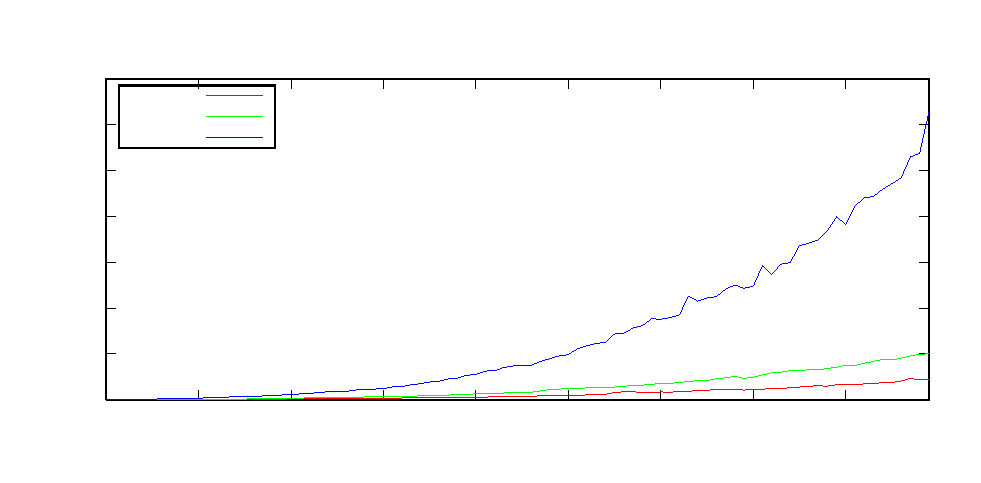
\includegraphics{grafo-completo-tiempo}}%
    \gplfronttext
  \end{picture}%
\endgroup

\end{figure}

\begin{figure}[H]
	% GNUPLOT: LaTeX picture with Postscript
\begingroup
  \makeatletter
  \providecommand\color[2][]{%
    \GenericError{(gnuplot) \space\space\space\@spaces}{%
      Package color not loaded in conjunction with
      terminal option `colourtext'%
    }{See the gnuplot documentation for explanation.%
    }{Either use 'blacktext' in gnuplot or load the package
      color.sty in LaTeX.}%
    \renewcommand\color[2][]{}%
  }%
  \providecommand\includegraphics[2][]{%
    \GenericError{(gnuplot) \space\space\space\@spaces}{%
      Package graphicx or graphics not loaded%
    }{See the gnuplot documentation for explanation.%
    }{The gnuplot epslatex terminal needs graphicx.sty or graphics.sty.}%
    \renewcommand\includegraphics[2][]{}%
  }%
  \providecommand\rotatebox[2]{#2}%
  \@ifundefined{ifGPcolor}{%
    \newif\ifGPcolor
    \GPcolorfalse
  }{}%
  \@ifundefined{ifGPblacktext}{%
    \newif\ifGPblacktext
    \GPblacktexttrue
  }{}%
  % define a \g@addto@macro without @ in the name:
  \let\gplgaddtomacro\g@addto@macro
  % define empty templates for all commands taking text:
  \gdef\gplbacktext{}%
  \gdef\gplfronttext{}%
  \makeatother
  \ifGPblacktext
    % no textcolor at all
    \def\colorrgb#1{}%
    \def\colorgray#1{}%
  \else
    % gray or color?
    \ifGPcolor
      \def\colorrgb#1{\color[rgb]{#1}}%
      \def\colorgray#1{\color[gray]{#1}}%
      \expandafter\def\csname LTw\endcsname{\color{white}}%
      \expandafter\def\csname LTb\endcsname{\color{black}}%
      \expandafter\def\csname LTa\endcsname{\color{black}}%
      \expandafter\def\csname LT0\endcsname{\color[rgb]{1,0,0}}%
      \expandafter\def\csname LT1\endcsname{\color[rgb]{0,1,0}}%
      \expandafter\def\csname LT2\endcsname{\color[rgb]{0,0,1}}%
      \expandafter\def\csname LT3\endcsname{\color[rgb]{1,0,1}}%
      \expandafter\def\csname LT4\endcsname{\color[rgb]{0,1,1}}%
      \expandafter\def\csname LT5\endcsname{\color[rgb]{1,1,0}}%
      \expandafter\def\csname LT6\endcsname{\color[rgb]{0,0,0}}%
      \expandafter\def\csname LT7\endcsname{\color[rgb]{1,0.3,0}}%
      \expandafter\def\csname LT8\endcsname{\color[rgb]{0.5,0.5,0.5}}%
    \else
      % gray
      \def\colorrgb#1{\color{black}}%
      \def\colorgray#1{\color[gray]{#1}}%
      \expandafter\def\csname LTw\endcsname{\color{white}}%
      \expandafter\def\csname LTb\endcsname{\color{black}}%
      \expandafter\def\csname LTa\endcsname{\color{black}}%
      \expandafter\def\csname LT0\endcsname{\color{black}}%
      \expandafter\def\csname LT1\endcsname{\color{black}}%
      \expandafter\def\csname LT2\endcsname{\color{black}}%
      \expandafter\def\csname LT3\endcsname{\color{black}}%
      \expandafter\def\csname LT4\endcsname{\color{black}}%
      \expandafter\def\csname LT5\endcsname{\color{black}}%
      \expandafter\def\csname LT6\endcsname{\color{black}}%
      \expandafter\def\csname LT7\endcsname{\color{black}}%
      \expandafter\def\csname LT8\endcsname{\color{black}}%
    \fi
  \fi
  \setlength{\unitlength}{0.0500bp}%
  \begin{picture}(9118.00,4320.00)%
    \gplgaddtomacro\gplbacktext{%
      \colorrgb{0.00,0.00,0.00}%
      \put(860,640){\makebox(0,0)[r]{\strut{}0}}%
      \colorrgb{0.00,0.00,0.00}%
      \put(860,1256){\makebox(0,0)[r]{\strut{}500}}%
      \colorrgb{0.00,0.00,0.00}%
      \put(860,1872){\makebox(0,0)[r]{\strut{}1000}}%
      \colorrgb{0.00,0.00,0.00}%
      \put(860,2487){\makebox(0,0)[r]{\strut{}1500}}%
      \colorrgb{0.00,0.00,0.00}%
      \put(860,3103){\makebox(0,0)[r]{\strut{}2000}}%
      \colorrgb{0.00,0.00,0.00}%
      \put(860,3719){\makebox(0,0)[r]{\strut{}2500}}%
      \colorrgb{0.00,0.00,0.00}%
      \put(980,440){\makebox(0,0){\strut{}10}}%
      \colorrgb{0.00,0.00,0.00}%
      \put(1854,440){\makebox(0,0){\strut{}20}}%
      \colorrgb{0.00,0.00,0.00}%
      \put(2728,440){\makebox(0,0){\strut{}30}}%
      \colorrgb{0.00,0.00,0.00}%
      \put(3601,440){\makebox(0,0){\strut{}40}}%
      \colorrgb{0.00,0.00,0.00}%
      \put(4475,440){\makebox(0,0){\strut{}50}}%
      \colorrgb{0.00,0.00,0.00}%
      \put(5349,440){\makebox(0,0){\strut{}60}}%
      \colorrgb{0.00,0.00,0.00}%
      \put(6223,440){\makebox(0,0){\strut{}70}}%
      \colorrgb{0.00,0.00,0.00}%
      \put(7097,440){\makebox(0,0){\strut{}80}}%
      \colorrgb{0.00,0.00,0.00}%
      \put(7971,440){\makebox(0,0){\strut{}90}}%
      \colorrgb{0.00,0.00,0.00}%
      \put(160,2179){\rotatebox{90}{\makebox(0,0){\strut{}Tamaño de la frontera de la CMF hallada}}}%
      \colorrgb{0.00,0.00,0.00}%
      \put(4868,140){\makebox(0,0){\strut{}$n$}}%
      \csname LTb\endcsname%
      \put(4868,4019){\makebox(0,0){\strut{}Grafo completo: Tamaño de las fronteras de las CMF halladas}}%
    }%
    \gplgaddtomacro\gplfronttext{%
      \csname LTb\endcsname%
      \put(1820,3556){\makebox(0,0)[r]{\strut{}Goloso}}%
      \csname LTb\endcsname%
      \put(1820,3356){\makebox(0,0)[r]{\strut{}Local}}%
      \csname LTb\endcsname%
      \put(1820,3156){\makebox(0,0)[r]{\strut{}Tab\'u}}%
    }%
    \gplbacktext
    \put(0,0){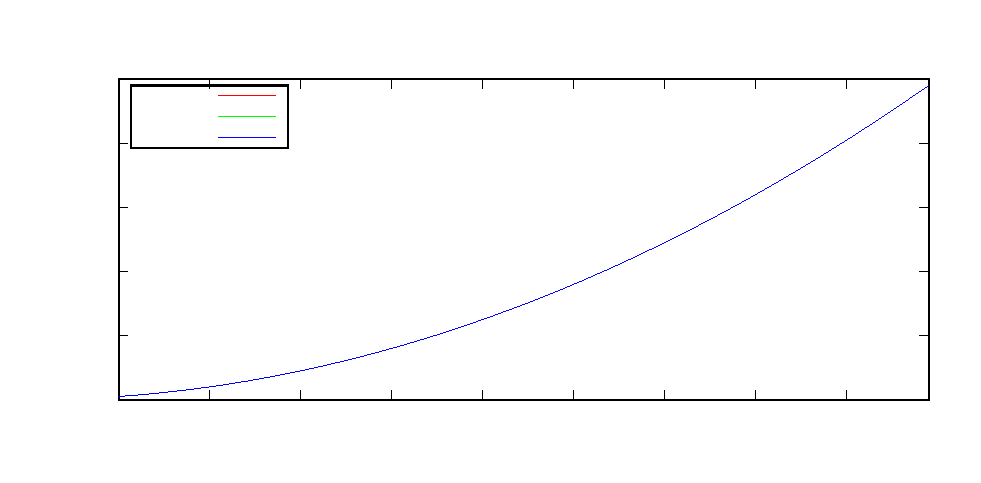
\includegraphics{grafo-completo-frontera}}%
    \gplfronttext
  \end{picture}%
\endgroup

\end{figure}


\subsection{Familia lattice I}

\begin{figure}[H]
	% GNUPLOT: LaTeX picture with Postscript
\begingroup
  \makeatletter
  \providecommand\color[2][]{%
    \GenericError{(gnuplot) \space\space\space\@spaces}{%
      Package color not loaded in conjunction with
      terminal option `colourtext'%
    }{See the gnuplot documentation for explanation.%
    }{Either use 'blacktext' in gnuplot or load the package
      color.sty in LaTeX.}%
    \renewcommand\color[2][]{}%
  }%
  \providecommand\includegraphics[2][]{%
    \GenericError{(gnuplot) \space\space\space\@spaces}{%
      Package graphicx or graphics not loaded%
    }{See the gnuplot documentation for explanation.%
    }{The gnuplot epslatex terminal needs graphicx.sty or graphics.sty.}%
    \renewcommand\includegraphics[2][]{}%
  }%
  \providecommand\rotatebox[2]{#2}%
  \@ifundefined{ifGPcolor}{%
    \newif\ifGPcolor
    \GPcolorfalse
  }{}%
  \@ifundefined{ifGPblacktext}{%
    \newif\ifGPblacktext
    \GPblacktexttrue
  }{}%
  % define a \g@addto@macro without @ in the name:
  \let\gplgaddtomacro\g@addto@macro
  % define empty templates for all commands taking text:
  \gdef\gplbacktext{}%
  \gdef\gplfronttext{}%
  \makeatother
  \ifGPblacktext
    % no textcolor at all
    \def\colorrgb#1{}%
    \def\colorgray#1{}%
  \else
    % gray or color?
    \ifGPcolor
      \def\colorrgb#1{\color[rgb]{#1}}%
      \def\colorgray#1{\color[gray]{#1}}%
      \expandafter\def\csname LTw\endcsname{\color{white}}%
      \expandafter\def\csname LTb\endcsname{\color{black}}%
      \expandafter\def\csname LTa\endcsname{\color{black}}%
      \expandafter\def\csname LT0\endcsname{\color[rgb]{1,0,0}}%
      \expandafter\def\csname LT1\endcsname{\color[rgb]{0,1,0}}%
      \expandafter\def\csname LT2\endcsname{\color[rgb]{0,0,1}}%
      \expandafter\def\csname LT3\endcsname{\color[rgb]{1,0,1}}%
      \expandafter\def\csname LT4\endcsname{\color[rgb]{0,1,1}}%
      \expandafter\def\csname LT5\endcsname{\color[rgb]{1,1,0}}%
      \expandafter\def\csname LT6\endcsname{\color[rgb]{0,0,0}}%
      \expandafter\def\csname LT7\endcsname{\color[rgb]{1,0.3,0}}%
      \expandafter\def\csname LT8\endcsname{\color[rgb]{0.5,0.5,0.5}}%
    \else
      % gray
      \def\colorrgb#1{\color{black}}%
      \def\colorgray#1{\color[gray]{#1}}%
      \expandafter\def\csname LTw\endcsname{\color{white}}%
      \expandafter\def\csname LTb\endcsname{\color{black}}%
      \expandafter\def\csname LTa\endcsname{\color{black}}%
      \expandafter\def\csname LT0\endcsname{\color{black}}%
      \expandafter\def\csname LT1\endcsname{\color{black}}%
      \expandafter\def\csname LT2\endcsname{\color{black}}%
      \expandafter\def\csname LT3\endcsname{\color{black}}%
      \expandafter\def\csname LT4\endcsname{\color{black}}%
      \expandafter\def\csname LT5\endcsname{\color{black}}%
      \expandafter\def\csname LT6\endcsname{\color{black}}%
      \expandafter\def\csname LT7\endcsname{\color{black}}%
      \expandafter\def\csname LT8\endcsname{\color{black}}%
    \fi
  \fi
  \setlength{\unitlength}{0.0500bp}%
  \begin{picture}(9118.00,4320.00)%
    \gplgaddtomacro\gplbacktext{%
      \colorrgb{0.00,0.00,0.00}%
      \put(740,640){\makebox(0,0)[r]{\strut{}0}}%
      \colorrgb{0.00,0.00,0.00}%
      \put(740,1256){\makebox(0,0)[r]{\strut{}100}}%
      \colorrgb{0.00,0.00,0.00}%
      \put(740,1872){\makebox(0,0)[r]{\strut{}200}}%
      \colorrgb{0.00,0.00,0.00}%
      \put(740,2487){\makebox(0,0)[r]{\strut{}300}}%
      \colorrgb{0.00,0.00,0.00}%
      \put(740,3103){\makebox(0,0)[r]{\strut{}400}}%
      \colorrgb{0.00,0.00,0.00}%
      \put(740,3719){\makebox(0,0)[r]{\strut{}500}}%
      \colorrgb{0.00,0.00,0.00}%
      \put(860,440){\makebox(0,0){\strut{}10}}%
      \colorrgb{0.00,0.00,0.00}%
      \put(1747,440){\makebox(0,0){\strut{}20}}%
      \colorrgb{0.00,0.00,0.00}%
      \put(2635,440){\makebox(0,0){\strut{}30}}%
      \colorrgb{0.00,0.00,0.00}%
      \put(3522,440){\makebox(0,0){\strut{}40}}%
      \colorrgb{0.00,0.00,0.00}%
      \put(4409,440){\makebox(0,0){\strut{}50}}%
      \colorrgb{0.00,0.00,0.00}%
      \put(5297,440){\makebox(0,0){\strut{}60}}%
      \colorrgb{0.00,0.00,0.00}%
      \put(6184,440){\makebox(0,0){\strut{}70}}%
      \colorrgb{0.00,0.00,0.00}%
      \put(7071,440){\makebox(0,0){\strut{}80}}%
      \colorrgb{0.00,0.00,0.00}%
      \put(7958,440){\makebox(0,0){\strut{}90}}%
      \colorrgb{0.00,0.00,0.00}%
      \put(160,2179){\rotatebox{90}{\makebox(0,0){\strut{}Tiempo (milisegundos)}}}%
      \colorrgb{0.00,0.00,0.00}%
      \put(4808,140){\makebox(0,0){\strut{}$n$}}%
      \csname LTb\endcsname%
      \put(4808,4019){\makebox(0,0){\strut{}Lattice I: Tiempo de ejecuci\'on}}%
    }%
    \gplgaddtomacro\gplfronttext{%
      \csname LTb\endcsname%
      \put(1700,3556){\makebox(0,0)[r]{\strut{}Goloso}}%
      \csname LTb\endcsname%
      \put(1700,3356){\makebox(0,0)[r]{\strut{}Local}}%
      \csname LTb\endcsname%
      \put(1700,3156){\makebox(0,0)[r]{\strut{}Tab\'u}}%
    }%
    \gplbacktext
    \put(0,0){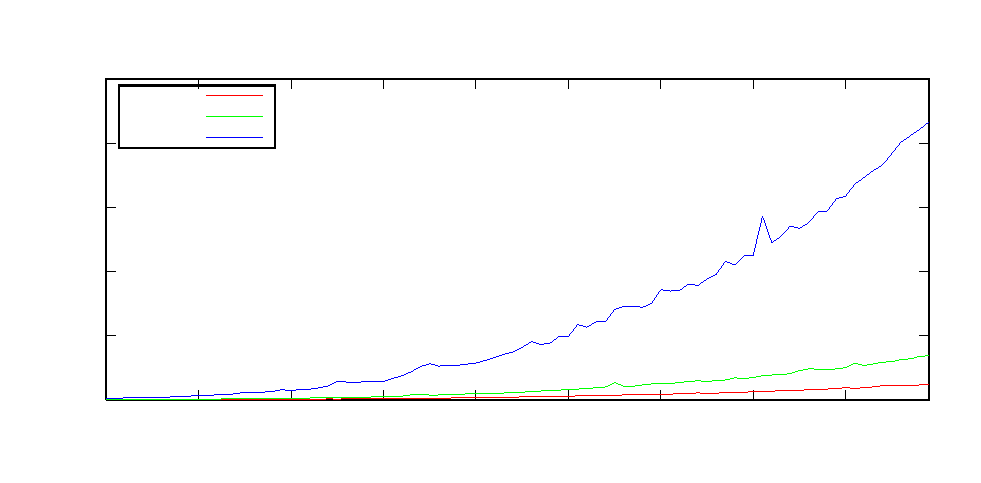
\includegraphics{lattice-i-tiempo}}%
    \gplfronttext
  \end{picture}%
\endgroup

\end{figure}

\begin{figure}[H]
	% GNUPLOT: LaTeX picture with Postscript
\begingroup
  \makeatletter
  \providecommand\color[2][]{%
    \GenericError{(gnuplot) \space\space\space\@spaces}{%
      Package color not loaded in conjunction with
      terminal option `colourtext'%
    }{See the gnuplot documentation for explanation.%
    }{Either use 'blacktext' in gnuplot or load the package
      color.sty in LaTeX.}%
    \renewcommand\color[2][]{}%
  }%
  \providecommand\includegraphics[2][]{%
    \GenericError{(gnuplot) \space\space\space\@spaces}{%
      Package graphicx or graphics not loaded%
    }{See the gnuplot documentation for explanation.%
    }{The gnuplot epslatex terminal needs graphicx.sty or graphics.sty.}%
    \renewcommand\includegraphics[2][]{}%
  }%
  \providecommand\rotatebox[2]{#2}%
  \@ifundefined{ifGPcolor}{%
    \newif\ifGPcolor
    \GPcolorfalse
  }{}%
  \@ifundefined{ifGPblacktext}{%
    \newif\ifGPblacktext
    \GPblacktexttrue
  }{}%
  % define a \g@addto@macro without @ in the name:
  \let\gplgaddtomacro\g@addto@macro
  % define empty templates for all commands taking text:
  \gdef\gplbacktext{}%
  \gdef\gplfronttext{}%
  \makeatother
  \ifGPblacktext
    % no textcolor at all
    \def\colorrgb#1{}%
    \def\colorgray#1{}%
  \else
    % gray or color?
    \ifGPcolor
      \def\colorrgb#1{\color[rgb]{#1}}%
      \def\colorgray#1{\color[gray]{#1}}%
      \expandafter\def\csname LTw\endcsname{\color{white}}%
      \expandafter\def\csname LTb\endcsname{\color{black}}%
      \expandafter\def\csname LTa\endcsname{\color{black}}%
      \expandafter\def\csname LT0\endcsname{\color[rgb]{1,0,0}}%
      \expandafter\def\csname LT1\endcsname{\color[rgb]{0,1,0}}%
      \expandafter\def\csname LT2\endcsname{\color[rgb]{0,0,1}}%
      \expandafter\def\csname LT3\endcsname{\color[rgb]{1,0,1}}%
      \expandafter\def\csname LT4\endcsname{\color[rgb]{0,1,1}}%
      \expandafter\def\csname LT5\endcsname{\color[rgb]{1,1,0}}%
      \expandafter\def\csname LT6\endcsname{\color[rgb]{0,0,0}}%
      \expandafter\def\csname LT7\endcsname{\color[rgb]{1,0.3,0}}%
      \expandafter\def\csname LT8\endcsname{\color[rgb]{0.5,0.5,0.5}}%
    \else
      % gray
      \def\colorrgb#1{\color{black}}%
      \def\colorgray#1{\color[gray]{#1}}%
      \expandafter\def\csname LTw\endcsname{\color{white}}%
      \expandafter\def\csname LTb\endcsname{\color{black}}%
      \expandafter\def\csname LTa\endcsname{\color{black}}%
      \expandafter\def\csname LT0\endcsname{\color{black}}%
      \expandafter\def\csname LT1\endcsname{\color{black}}%
      \expandafter\def\csname LT2\endcsname{\color{black}}%
      \expandafter\def\csname LT3\endcsname{\color{black}}%
      \expandafter\def\csname LT4\endcsname{\color{black}}%
      \expandafter\def\csname LT5\endcsname{\color{black}}%
      \expandafter\def\csname LT6\endcsname{\color{black}}%
      \expandafter\def\csname LT7\endcsname{\color{black}}%
      \expandafter\def\csname LT8\endcsname{\color{black}}%
    \fi
  \fi
  \setlength{\unitlength}{0.0500bp}%
  \begin{picture}(9118.00,4320.00)%
    \gplgaddtomacro\gplbacktext{%
      \colorrgb{0.00,0.00,0.00}%
      \put(860,640){\makebox(0,0)[r]{\strut{}0}}%
      \colorrgb{0.00,0.00,0.00}%
      \put(860,1153){\makebox(0,0)[r]{\strut{}500}}%
      \colorrgb{0.00,0.00,0.00}%
      \put(860,1666){\makebox(0,0)[r]{\strut{}1000}}%
      \colorrgb{0.00,0.00,0.00}%
      \put(860,2180){\makebox(0,0)[r]{\strut{}1500}}%
      \colorrgb{0.00,0.00,0.00}%
      \put(860,2693){\makebox(0,0)[r]{\strut{}2000}}%
      \colorrgb{0.00,0.00,0.00}%
      \put(860,3206){\makebox(0,0)[r]{\strut{}2500}}%
      \colorrgb{0.00,0.00,0.00}%
      \put(860,3719){\makebox(0,0)[r]{\strut{}3000}}%
      \colorrgb{0.00,0.00,0.00}%
      \put(980,440){\makebox(0,0){\strut{}10}}%
      \colorrgb{0.00,0.00,0.00}%
      \put(1854,440){\makebox(0,0){\strut{}20}}%
      \colorrgb{0.00,0.00,0.00}%
      \put(2728,440){\makebox(0,0){\strut{}30}}%
      \colorrgb{0.00,0.00,0.00}%
      \put(3601,440){\makebox(0,0){\strut{}40}}%
      \colorrgb{0.00,0.00,0.00}%
      \put(4475,440){\makebox(0,0){\strut{}50}}%
      \colorrgb{0.00,0.00,0.00}%
      \put(5349,440){\makebox(0,0){\strut{}60}}%
      \colorrgb{0.00,0.00,0.00}%
      \put(6223,440){\makebox(0,0){\strut{}70}}%
      \colorrgb{0.00,0.00,0.00}%
      \put(7097,440){\makebox(0,0){\strut{}80}}%
      \colorrgb{0.00,0.00,0.00}%
      \put(7971,440){\makebox(0,0){\strut{}90}}%
      \colorrgb{0.00,0.00,0.00}%
      \put(160,2179){\rotatebox{90}{\makebox(0,0){\strut{}Tamaño de la frontera de la CMF hallada}}}%
      \colorrgb{0.00,0.00,0.00}%
      \put(4868,140){\makebox(0,0){\strut{}$n$}}%
      \csname LTb\endcsname%
      \put(4868,4019){\makebox(0,0){\strut{}Lattice I: Tamaño de las fronteras de las CMF halladas}}%
    }%
    \gplgaddtomacro\gplfronttext{%
      \csname LTb\endcsname%
      \put(1820,3556){\makebox(0,0)[r]{\strut{}Goloso}}%
      \csname LTb\endcsname%
      \put(1820,3356){\makebox(0,0)[r]{\strut{}Local}}%
      \csname LTb\endcsname%
      \put(1820,3156){\makebox(0,0)[r]{\strut{}Tab\'u}}%
    }%
    \gplbacktext
    \put(0,0){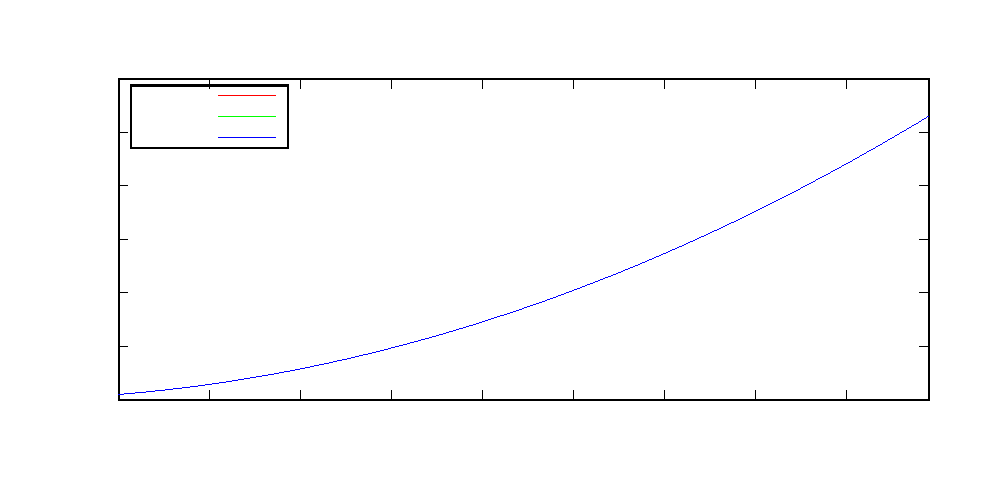
\includegraphics{lattice-i-frontera}}%
    \gplfronttext
  \end{picture}%
\endgroup

\end{figure}

\end{document}